\clearpage

\section{MC Samples and event weighting}
\label{sec:mcsample}
%-------------------------------------------------------------------------------
% *refraseMT*
The samples used are divided into two main groups: Standard Model (SM) background and beyond SM signal. The SM background includes the QCD multijet samples, produced with a falling $\pt$ spectrum. The beyond SM signals are $W'\to WZ\to q\bar{q}'q\bar{q}$, $Z'\to t\bar{t}$ where both top quarks  decay according to $t\to W(\to q\bar{q}')b$, and RS-Graviton $\to hh \to b\bar{b}b\bar{b}$, i.e. final states have only jets in all the samples. The details of the samples are given in Table \ref{tab:mcsamples}; the masses considered span from 0.5 to 5 TeV to improve and diversify the kinematic space covered.


\begin{table}[b]
\centering
%\hspace*{-3em}
\begin{tabular}{l|lllr}  
% \toprule
\hline
\hline
Process & ME Generator & ME PDFs &  UE Tune & Resonance Masses\\
  & \& Fragmentation &  & & \\

\hline
QCD multijet &Pythia 8&NNPDF23LO & A14& N/A \\
\hline
$W'\to WZ$ &Pythia 8&NNPDF23LO & A14& 1.5, 2.5, 3, 4, 5 TeV \\
\cline{1-1}
$Z'\to t\bar{t}$ &Pythia 8&NNPDF23LO & A14& 1.5, 1.75, 2.5, 3, 4, 5 TeV \\
\cline{1-1}
$G_{RS} \to hh(\to b\bar{b})$ &Pythia 8&NNPDF23LO & A14& 0.5, 1, 1.5, 2, 2.5, 3 TeV\\
\cline{1-1}
$W' \to \tilde{W}\tilde{W}$ &Pythia 8&NNPDF23LO & A14& 1.5, 2.5, 3, 4, 5 TeV \\
with $m_{\tilde{W}}=m_t$ & & & & \\
\hline
\hline
% \bottomrule
\end{tabular}
\caption[Overview of the Monte Carlo Samples used]{Overview of the Monte Carlo Samples used. The first line shows QCD standard model process, the second, the third and the forth the beyond SM samples considered; the last line the ``massive $W/Z$'' sample.}
\label{tab:mcsamples}
% \end{center}
\end{table}
The performance of substructure observables is evaluated using QCD rejection for the same signal efficiency. While the $p_{\mathrm{T}}$ distribution of the multi-jet sample falls exponentially, the $p_{\mathrm{T}}$ of the signal samples features characteristic Jacobian peaks related to the resonance masses. To avoid any bias in the comparison, the signal sample is given weights such that the truth $p_{\mathrm{T}}$ distribution of the leading jet matches the one of the background sample (see Figure \ref{fig:p_T} in the Appendix). Furthermore, the spectrum is split into six different $p_{\mathrm{T}}$ regions to study the behaviour with rising energy.






% \newpage
%-------------------------------------------------------------------------------
\clearpage
\section{Object Definition}
\label{sec:objdef}
%-------------------------------------------------------------------------------

This Section gives an overview of the objects used for the observables based on subjet-assisted tracks, i.e., the large-radius jet mass and jet substructure observables derived from Energy Correlation Functions and n-subjettiness, as they are used by default within ATLAS.
% , the next Section will give the details of the modified approach of the subjet-assisted techniques.

\subsection{Standard Large-Radius Jet}


Large-radius jet, or large-$R$ jets used in this study are jets constructed with a radius parameter of the reclustering algorithm $R=1$ for those built using the anti-k$_t$ algorithm~\cite{antiktalgo}. 



Since the active area of this jets is typically six times bigger than their counterparts of $R=0.4$, further techniques are required to control the effect of contamination from pile up (PU) of additional $pp$ interactions in the same or preceding bunch crossing and of the Underlying Event (UE). To remove these additional, a trimming algorithm with standard ATLAS parameters~\cite{art35} is used throughout this note unless specified otherwise. Its parameters are summarised in Appendix~\ref{sec:trimming}. 
Other common choices are \textit{Split-Filtering} and \textit{Pruning}~\cite{substructure1}.

The selection applied to \larger jets is typical for many Beyond the Standard Model searches: $p_T>$ 250 GeV and $|\eta|<$ 2.0.
No other requirements were made for the purpose of the performance studies here shown if not stated differently, e.g. the mass cut selection.


\subsubsection{Calorimeter Mass}

The trimmed collection of topo-clusters from the large-$R$ jet is then used to reconstruct properties of the jet such as the jet mass. The \textit{calorimeter mass} $\mcal$ is a widely used variable which takes as input the topo-cluster information. Given that each topo-cluster $i$ has 3D information on the energy deposit, $E_i$, $\eta$ and $\phi$, the mass can be simply calculated from 4-vector properties:
$$\mcal=\sqrt{\left(\sum_{i\in J}E_i\right)^2-\left(\sum_{i\in J}p_{T,i}\right)^2} $$
where $o$ labels the topoclusters of the trimmed large-$R$ jet $J$ and the topoclusters are assumed massless.

\subsubsection{Track Mass}
\label{sec:tracks}
There are advantages and disadvantages when using tracks for \larger jet mass reconstruction, inherited both from the detector experimental properties and from the underlying physical processes. The track mass $m^\textrm{trk}$ is calculated summing up the 4-momenta of tracks which passed the selection and are ghost-associated to the trimmed jet.
\\ 
Main advantages of $m^\textrm{trk}$ are: performance of angular separation and the association of the tracks to the primary vertex for rejection of soft radiation background. \\
An important disadvantage of $m^\textrm{trk}$ comes from the complete blindness of the tracker system to the neutral component (mostly $\pi^0$'s) of the jet. As seen in Figure~\ref{fig:trackandcalo}, the track mass (red distribution) is not only shifted towards lower values than the calorimeter mass (green distribution), but its width also degrades. 


\begin{figure}[!ht]
  \centering
      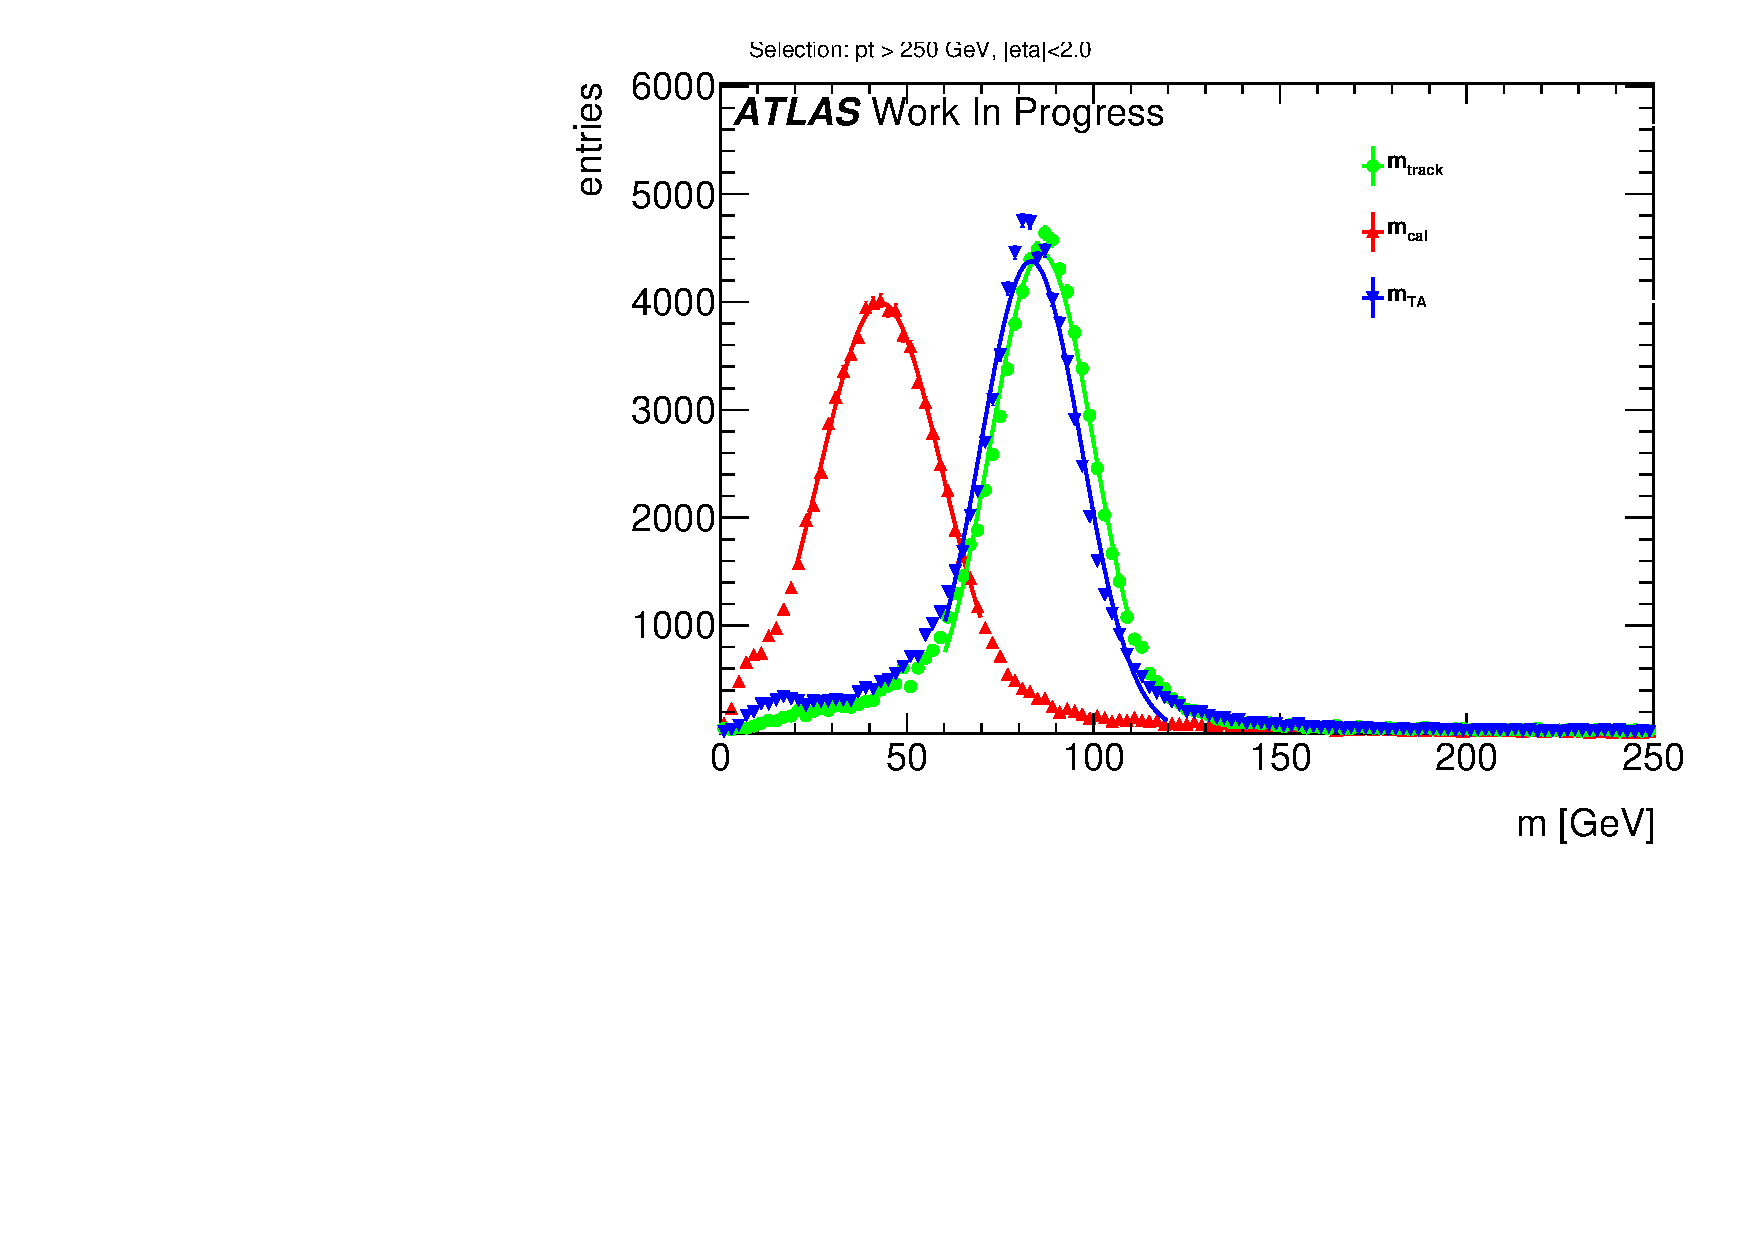
\includegraphics[width=0.7\textwidth]{jet_part/1cfrt_h_TrackJets_m.pdf}
  \caption[Mass distribution for $W/Z$ decays]{Mass distribution for $W/Z$ decays: in green the $\mcal$ in red the $m^\textrm{trk}$ and in blue the $\mta$. }
  \label{fig:trackandcalo}
\end{figure}


\subsubsection{Track-Assisted Mass ($\mta$)}
The track-assisted mass $\mta$ was one of the first attempts within ATLAS to combine the information form the tracker system and from the calorimeter to reconstruct the \larger jet mass~\cite{art35}, however, it has been proposed long before that~\cite{bib:schaetzel,bib:tweedie}. It is defined as $\mta=\frac{p_T^\textrm{calo}}{p_T^\textrm{trk}}\times m^\textrm{trk}$, where the $p_T^\textrm{trk}$ and the $m^\textrm{trk}$ are calculated from the tracks which are associated to the large-radius jet, adding up their 4-momenta (hence exploiting the superior angular resolution of the tracker system); the $p_T^\textrm{calo}$ is the transverse momentum as measured from the calorimeter system. The ratio $p_T^\textrm{calo}/p_T^\textrm{trk}$ restores the fraction of the missing neutral component in the $m^\textrm{trk}$.
The $\mta$ has a better performance on the reconstruction of boosted objects such as $W/Z$ in the extreme kinematic regime ($\sim $ 1 TeV) and above in the transverse momentum of the decaying electroweak object. Another advantage of this observable are its the systematic uncertainties: in particular jet mass scale and jet mass resolution uncertainty on $\mta$ can be estimated by propagating the track reconstruction uncertainties and calorimeter-jet $\pt$ uncertainties through the definition of the variable given above. The tracking-related uncertainties are smaller for $\mta$ rather than $\mcal$ because a larger extent of the uncertainty cancels in the ratio $m^\textrm{trk}/p_T^\textrm{trk}$.
Apart all of these advantages, the track-assisted mass hits its limits at intermediate transverse momentum regimes and below ($\pt < 1 $ TeV) for $W$ jets,  and throughout the whole kinematic space for Higgs and top quarks.
A full description of \mta is given in Ref.~\cite{art35}.



\subsection{The Track-Assisted Subjet Mass ($\mtas$)}\label{subsec:mtas_def}
In the following, the final algorithm to reconstruct the mass of \larger jets from subjet-assisted tracks is presented: the \textit{track-assisted subjet mass} ($\mtas$). The optimal choice of inputs to \mtas and other algorithmic details are the result of an optimisation, which will not be detailed here, except for the most striking results, which are summarised in Section~\ref{sec:alternate}.

The main idea behind \mtas to correct the energy scale of tracks per-subjet takes inspiration from \mta. The neutral fraction missed by the tracker, in fact, varies stochastically not only on a per-jet basis, but also on a per-subjet basis, since each quark follows a different parton showering and hadronization process, which to first order factorise.


\subsubsection{Observable Definition: Inputs}
\label{sec:tasinputs}
There are two inputs to the $\mtas$: tracks and subjets. The definition of the standard inputs are give here; alternative approaches are given in Section \ref{sec:alternate}.

\paragraph{Tracks}
Only the tracks that satisfy the quality criteria and primary vertex association, described in the appendix \ref{sec:tracks}, are used.
The tracks are additionally required to be ghost-associated to the subjets of the trimmed jet; namely only the subjets which survived the trimming procedure and are described in the next paragraph.
Ghost-association provides a clear correspondence of tracks to the subjets set and was therefore preferred to other kind of assignments like angular matching.


\paragraph{Subjets}
In the \mtas algorithm, the standard trimming procedure at ATLAS is applied, which uses the k$_t$ reclustering algorithm with $R=0.2$, with the transverse momentum ratio $f_{\rm cut}$ of 5\%.


\subsubsection{Observable Definition: Algorithm}
\label{sec:tasalgo}
\label{sec:tas}
There are two ways of subjet assisting the tracks for the calculation of the $\mtas$: assisting track-jets by calibrating their invariant mass, or assisting single tracks changing their \pt. The former approach was the first tried historically, and all results related to \mtas are obtained with it. The latter approach is found to be equivalent to the first~\cite{presentation}, as indicated for $W$ jets in Figure~\ref{fig:sascha}). For jet substructure observables, however, only the approach assisting the \pt scale of single tracks can be used.


\begin{figure}[!ht]
  \centering
      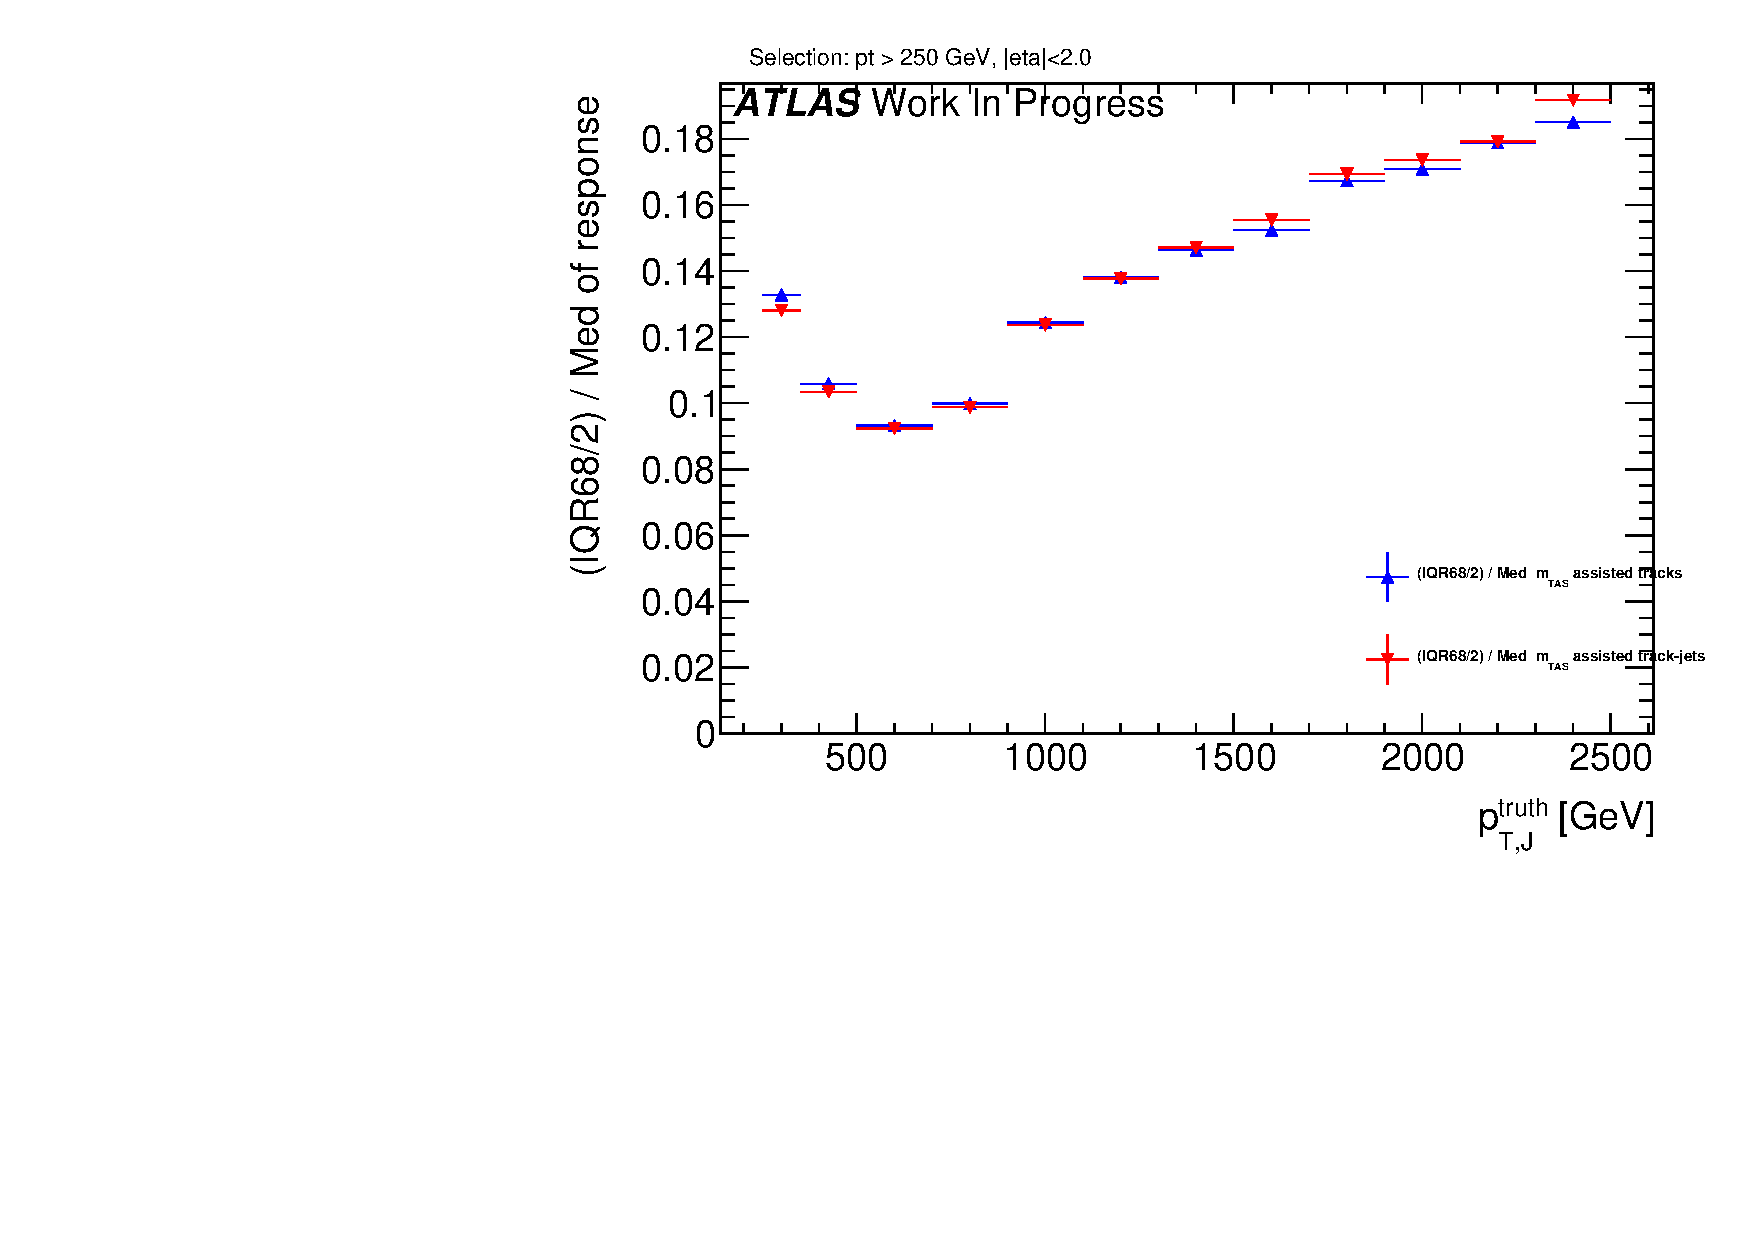
\includegraphics[width=0.55\textwidth]{jet_part/71graphcftr_h_JetRatio_mJ12CALOIQRoMwsecondApproach.pdf}
  \caption[Equivalence of approaches]{Performance of the $\mtas$ variable for the two approaches described in this Section: assisting track-jets (red) and assisting single tracks (blue) for $W$ jets. They are performing almost identically throughout the entire spectrum of transverse momentum. For the computation of the track-assisted subjet variable presented in this document, the former method is being used, because of simplicity of implementation and higher versatility; for the computation of the subjet assisted substructure variables the latter one is used. The y-axis is explained in the following Section.}
  \label{fig:sascha}
\end{figure}


\paragraph{Assisting Track-Jets}
The tracks are the ones ghost-associated to the subjets (SJ); however, tracks which fall inside the area of the large-$R$ jet and pass all other selection criteria except for the subjets area, are still likely to come from the hard-scattering. They are associated to the closest subjets through $\Delta R$ association. Thus, each subjet will have tracks associated via ghost-association, and at maximum 5\% of others via $\Delta R$. This set of tracks will be referred to as a ``custom'' Track-Jet or TJ in the following. The association procedure is schematically depicted in Fig.~\ref{fig:mtas1}.

\begin{figure}[!ht]
  \centering
      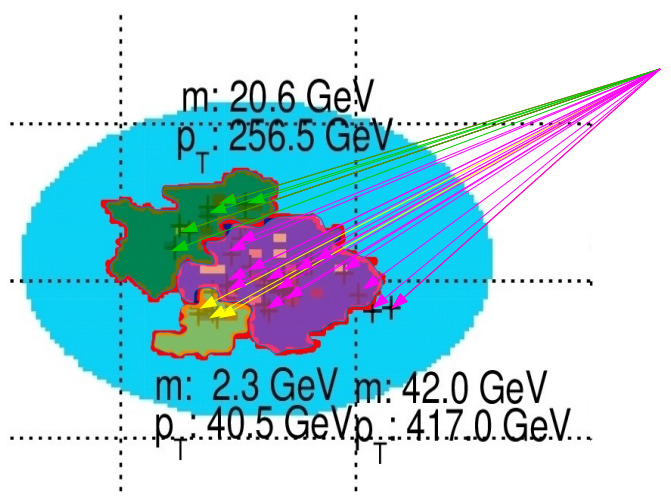
\includegraphics[width=0.6\textwidth]{jet_part/mtas/mtas.png}
  \caption[Pictorial event display]{Pictorial event display showing the $\eta$ $\phi$ region of a large-$R$ anti-k$_t$ trimmed jet, (in blue the catchment area of the anti-k$_t$) showing the different k$_t$ subjets: they are highlighted in green, fuchsia and yellow. The associated track-jets (here indicated as arrows pointing the calorimeter area) are coloured with the same colour of the correspondent subjet. Some tracks associated with $\Delta R$ procedure can be seen in the fuchsia subjet. The transverse momenta and mass values are also shown for the subjets.}
  \label{fig:mtas1}
\end{figure}

At this point, the one-to-one correspondence is preserved (for each SJ there is one and only one TJ. Taking inspiration from the formula $\mta=p_T^\textrm{calo}/p_T^\textrm{trk}\times m^\textrm{trk}$, the equivalent at subjet level should be
$$\mtas="\sum_{\rm SJ}"\frac{p_T^{\rm SJ}}{p_T^{\rm TJ}}\times m^{\rm TJ}\,,$$
where the summation symbol between quotation marks symbolizes that the sum is taken at 4-vector level: subjet's 4-vector itself needs to be modified and not only its mass. Denoting $p_\mu^{\rm TJ}$ as the Lorentz vector of the track-jet, its subjet-assistance is defined as 
$$p_\mu^{\rm TJ} = \spvec{m^{\rm TJ};p_T^{\rm TJ};\eta^{\rm TJ};\phi^{\rm TJ}} \to p_\mu^\textrm{TA}=\spvec{m^{\rm TJ}\times\frac{p_T^{\rm SJ}}{p_T^{\rm TJ}} ;p_T^{\rm SJ};\eta^{\rm TJ};\phi^{\rm TJ}}\,,$$
where $p_\mu^\textrm{TA}$ is the 4-vector of the track-assisted subjet. Labelling the $i$-th track-jet of the $N$ ones present in the large-$R$ jet,
\begin{equation}\label{eq:foursum}
\mtas=\sqrt{\left(\sum_i^N p^\textrm{TA}_i \right)_\mu \left(\sum_i^N p^\textrm{TA}_i \right)^{_\mu}}
\end{equation}
is defined.


\paragraph{Assisting Single Tracks}

Subjet-assistance is now applied on single track rather than the whole track-jet and on the transverse momentum, not the mass.
The correction reads:
$$
p_\mu^\textrm{trk} = \spvec{m^\textrm{trk};p_T^\textrm{trk};\eta^\textrm{trk};\phi^\textrm{trk}} \to p_\mu^\textrm{TA}=\spvec{m^\textrm{trk} ;p_T^\textrm{trk} \times\frac{p_T^{\rm SJ}}{p_T^{\rm TJ}};\eta^\textrm{trk};\phi^\textrm{trk}}
$$
The correction factor $\frac{p_T^{\rm SJ}}{p_T^{\rm TJ}}$ refers to the $\pt$ of the track-jet that the tracks is part of, and the subjet associated to that track-jet, as above.
As before, these four-momenta are then summed together according to Eq.~(\ref{eq:foursum}), with the only difference that the label $i$ refers to single tracks now.

An important remark is that, in the case of a large-$R$ jet with only one subjet, $\mtas$ has exactly the same definition of the $\mta$. This implies, since the angular separation of the decay product scales inversely with $\pt$, that the performance of \mtas should approach the one of $\mta$ at very high transverse momenta. The space for improvement is precisely in the low to intermediate $\pt$ regime.




\subsection{The Combined Mass}
\label{subsec:comb}


Since \mcalo is not explicitly used in \mta and \mtas, it is possible to improve the performance of the mass reconstruction by creating a new observable which combines both mass definitions.



\subsubsection{Combination of $\mta-\mcal$}

For the $\mta-\mcal$ combination~\cite{art35}, the observable are assumed to be statistically  independent, and combined using the uncertainty-weighted mean:
\begin{equation}
\mcomb\equiv a\times \mcal + b \times \mta\,,
\end{equation}
with 
\begin{equation}
a\equiv\frac{\sigma_\textrm{calo}^{-2}}{\sigma_\textrm{calo}^{-2}+\sigma_\textrm{TA}^{-2}} \qquad{\rm and}\qquad b\equiv\frac{\sigma_\textrm{TA}^{-2}}{\sigma_\textrm{calo}^{-2}+\sigma_\textrm{TA}^{-2}}\,.
\label{eq:mtacomb}
\end{equation}
Here, $\sigma_\textrm{calo}$ and $\sigma_\textrm{TA}$ are the $\mcal$'s and $\mta$'s resolution functions, computed from the mass response distribution, where the response is defined as the ratio of the observable calculated at detector level divided by its value determined at particle level; the sigma parameter corresponds to the width of the distribution, which is estimated using the InterQuantile range, as discussed in Section~\ref{sec:FoM}.

\subsubsection{Combination of $\mtas-\mcal$ }

The main difference between the $\mtas$ and $\mta$ when it comes to combination with \mcal is that the correlation of \mtas with \mcal is expected to be somewhat higher since the $\mtas$ uses subjet level information. This can be seen e.g. in  Figure~\ref{fig:mcomb2} and in Figure~\ref{fig:mcomba2} in Appendix~\ref{sec:kinematic}. The approach taken here is to take into account the (linear) correlation through the formula:
\begin{equation}
\begin{gathered}
\mcombtas= w\times\mcal + (1-w)\times\mtas,\\
w=\frac{\sigma_\textrm{TAS}^2-\rho\sigma_\textrm{calo}\sigma_\textrm{TAS}}{\sigma_\textrm{calo}^2+\sigma_\textrm{TAS}^2-2\rho\sigma_\textrm{calo}\sigma_\textrm{TAS}}\,,
\end{gathered}
\label{eq:mtascomb}
\end{equation}
% 
where now $\mcombtas$ is the new $\mtas-\mta$ combination. Alternatively, this can be written symmetrically as:
\begin{equation}
\begin{gathered}
\mcombtas= a\times\mcal + b\times\mtas,\\
a=\frac{\sigma_\textrm{TAS}^2-\rho\sigma_\textrm{calo}\sigma_\textrm{TAS}}{\sigma_\textrm{calo}^2+\sigma_\textrm{TAS}^2-2\rho\sigma_\textrm{TAS}\sigma_\textrm{calo}}\qquad b=\frac{\sigma_\textrm{calo}^2-\rho\sigma_\textrm{calo}\sigma_\textrm{TAS}}{\sigma_\textrm{calo}^2+\sigma_\textrm{TAS}^2-2\rho\sigma_\textrm{TAS}\sigma_\textrm{calo}}\,,
\end{gathered}
\end{equation}
which reduces to Eq.~\eqref{eq:mtacomb} after simple algebra for the case when $\rho=0$. Of course, this value can be set to the value of the specific sample considered, or to an average of 0.3 if one wants to give a definition generally valid for all the cases considered; in this case, the performance would be slightly sub-optimal.

The algorithm of producing $\mcombtas$ is summarised as follows:
\begin{enumerate}
 \item For the given sample, the $\mtas$ and $\mcal$ are calculated;
 \item The mass responses are also produced for the given ranges of $\pt$;
 \item For each of these responses, the value of the $\frac{68\% \: \textrm{IQnR}}{2}$ (described in Section~\ref{sec:FoM} and denoted as $\sigma$ in Eq.~\eqref{eq:mtascomb}) is calculated and stored;
 \item The average correlation factor of 0.3, an average value for the samples considered is assumed;
 \item $\mcombtas$ is calculated according to Eq.~\eqref{eq:mtascomb} using the values stored in step 3.
\end{enumerate}
In this note, the IQnR weights are produced for each sample specifically. In order to give a sample-independent definition of the $\mcombtas$, following also the procedure adopted for the $\mcomb$, these weights could be taken from a QCD multijet sample and applied indiscriminately to the particular case. The performance would be somewhat sub-optimal in this case.

Throughout the results presented in the following Sections, both \mcomb and \mcombtas  were calculated with sample-specific weights. Quantitative statements between them would still hold in the case of QCD weights. However, when confronting e.g. $\mtas$ with \mcomb, it has to be kept in mind that in this case the performance of \mcomb is overestimated.

\begin{figure}[!ht]
  \centering
      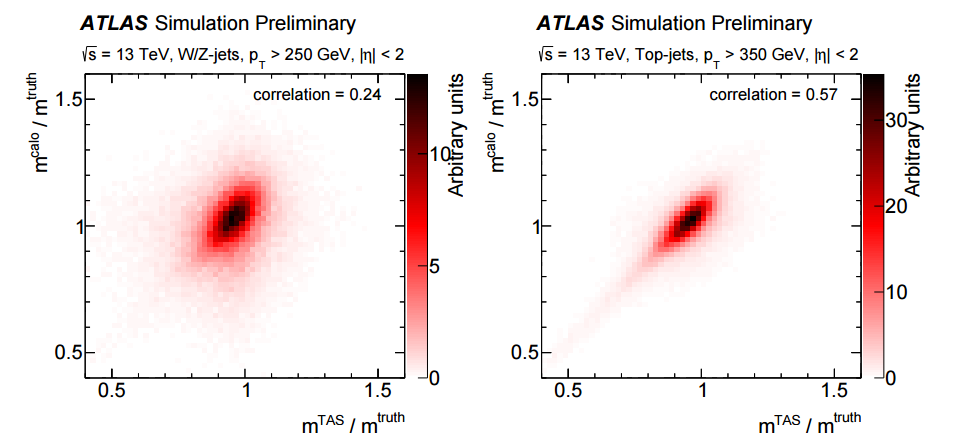
\includegraphics[width=0.7\textwidth]{jet_part/mcomb/mcomb2.png}
  \caption[$\mcal$ and $\mtas$ correlation plots]{The response of the detector in \mtas versus \mcalo, on the left for $W/Z$ jets and on the right for tops jets, from~\cite{art35}. The correlation is more pronounced for top jets.}
  \label{fig:mcomb2}
\end{figure}



